\documentclass[12pt,notitlepage]{article}

\usepackage{hyperref}
\hypersetup{colorlinks = true, linkcolor = blue}

\usepackage{graphicx}
\graphicspath{{./images/}}

% To use glossaries uncomment below

%\usepackage[toc]{glossaries}
%\makeglossaries
%\include{<glossaryfilename>}

\begin{document}

\title{Android}
\author{}
\date{}
\maketitle

%\tableofcontents
%\newpage

\section{Introduction}

Welcome to the Android coffee shop!

In these notes we use the analogy of a coffee shop in order to explain and
think about the android system and how it works.

To start checkout the overview \hyperref[sec:overview]{here}.

There is no best path to study these notes, however they have been linked
together in the order that they were created. For a full index see below:


\section{Overview}\label{sec:overview}

\href{https://developer.android.com/guide/index.html}{source}

\subsection{App Fundamentals}

The \textbf{.apk} extension refers to the compiled ``archive'' file used to install the
app.

Every app runs in its own virtual machine (VM) that's known as its app sandbox.

%\begin{figure}[h]
%    \centering
%    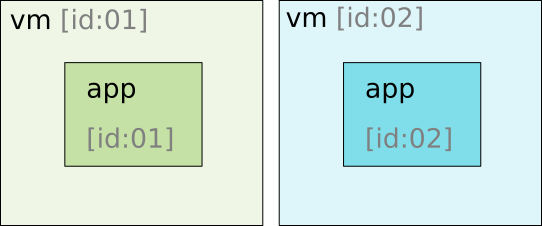
\includegraphics{app_sandbox.png}
%    \caption{Figure depicting the app sandbox}\label{fig:app_sandbox}
%\end{figure}

These VM processes are self contained and managed by the user account for the
app and the system.

This app's user account is given specialised permissions that the app requests,
but it is not known by the app itself!

You can view it as the app's guardian or wrangler.

So to clarify:
\begin{itemize}
    \item every app has a user account registered on the underlying Linux system
    \item this user account owns the vm process within which the app runs
    \item the app is contained in the vm controlled by both the system and the app user account
\end{itemize}

Whenever an app component is started, it activates the app process owned by the
user account. This is shutdown when no longer needed or by the system when it
needs to recover memory.

\subsection{Principle of Least Priviledge}

The user account is the thing that is given or denied permissions. For example,
if your app wants access to the camera, the user account is granted those
permissions by the system which then lets the app access the camera.

The \emph{Principle of Least Priviledge} basically means that an app only has
access to the base minimum it needs to work and no more!

These permissions are specified in the ``AndroidManifest.xml'' and is used to
grant the app permissions either at install time or run-time.

\subsection{Sharing data between apps?}

Because of how the Android system works, there are two ways to share data
between two different apps: the hard(er) way and the easy way.

\subsubsection{The harder way}
\begin{itemize}
    \item apps share a user account (id)
    \item same user account means same vm process
\end{itemize}

How: both apps must be signed using the same certificate

\subsubsection{The easy way}
\begin{itemize}
    \item apps have different user accounts
    \item simpler ad-hoc sharing
\end{itemize}

How: requesting permissions from the app user account


\section{Components}

Now that we have the building and owner for our app we can look at all the
stuff it is able to offer the customers and community. After all, no app is an
island and correctly understanding the different types of app components will
allow our app to have great synergy with the rest of the Android system.

There are 4 main types of components namely: activities, services, broadcast
receivers, and content providers.

Each component is defined as an ``entry point'' into the app and can be viewed as
ways for customers to interact with our coffee shop. The image below will make
more sense as we go into detail about each different type.

%\begin{figure}[h]
%    \centering
%    \includegraphics{shop.png}
%    \caption{Diagram of the proverbial shop}\label{fig:shop}
%\end{figure}

Each component has its own special lifecycle in terms of when they run.

\subsection{Activities}

The activities of an app each define one clear, well, activity.

These are generally used to directly interact with a user and can be used as an
entry point by itself. For example, you can view an activity as a barista that
is specialised to do one thing and do it really well. 

When you first enter the coffee shop you will encounter the ``order a coffee''
activity which is followed by the ``pay for coffee'' activity. In this coffee
shop the ordering and paying for coffee is handled separately so that if a
customer wants to just order a coffee and then dash out for a bit before
paying, they won't have to re-order coffee before paying for it.

\subsubsection{System \and User interaction}

Since activities are only used with user interaction they need to clearly
communicate to the system what they are currently doing so that the system
doesn't kill them when it needs to recover memory.

There are 4 main things the activity relays to the system:

\begin{enumerate}
    \item What's currently on the screen
    \item The user might return to this activity please don't kill it
    \item This activity is done, kill it and clean-up
    \item Allowing user to flow to other apps
\end{enumerate}

Point number 3 is interesting because the activity/app can't terminate itself, but
has to request the system to do so.

These 4 states can be summed up with the following diagram below.
%\appendix

\end{document}
